\documentclass[12pt]{article}
 
\usepackage[margin=1in]{geometry} 
\usepackage{amsmath,amsthm,amssymb}
\usepackage{graphicx}
\usepackage{bbold}
\usepackage{multirow}

\newcommand{\N}{\mathbb{N}}
\newcommand{\Z}{\mathbb{Z}}
\newcommand{\E}{\mathbb{E}}
\newcommand{\Prob}{\text{Prob}}


\begin{document}
\title{\large \textbf{The TANK Model with CBDC, Bank and Dollarization}}
\date{}
\maketitle
\section{Model without Dollarization}
This model is an extension of the TANK model in a small open economy, with CBDC and a monopolistic competitive bank sector. Deposit, cash and CBDC provide liquidity service and decrease the transaction cost. Banks take deposits from unconstrained households and invest in intermediate firms; constrained households do not have access to bank services and can only hold cash or CBDC. 

\subsection{Households}
The consumption bundle is defined as follows:
\begin{align*}
c_t = [\gamma^{\frac{1}{\eta}}c_{Ht}^{\frac{\eta-1}{\eta}}+(1-\gamma)^{\frac{1}{\eta}}c_{Ft}^{\frac{\eta-1}{\eta}}]^{\frac{\eta}{\eta-1}}, 
\end{align*}
where $c_{Ht}$ and $c_{Ft}$ denote consumption of domestic and foreign final good respectively. $\gamma$ is the home bias. The representative household decides how to allocate her consumption expenditure between domestic and foreign goods.

By solving the static optimization problem, the optimal consumption of domestic and foreign final goods can be solved as 
\begin{align*}
c_{Ht} &= \gamma(\frac{P_{Ht}}{p_t})^{-\eta}, \\
c_{Ft} &= (1-\gamma)(\frac{P_{Ft}}{p_t})^{-\eta}, 
\end{align*}
where $p_t$ is the domestic CPI, i.e., the price of one unit of consumption: 
\begin{align*}
p_t = [\gamma P_{Ht}^{1-\eta}+(1-\gamma)P_{Ft}^{1-\eta}]^{\frac{1}{1-\eta}}.
\end{align*}
In a small open economy, the price of the foreign good coincides with the foreign CPI $p_t^*$, adjusted by the nominal exchange rate $e_t$:
\begin{align*}
P_{Ft} = e_tp_t^*
\end{align*}
The real exchange rate is defined as the ratio of the foreign and domestic price levels, where the foreign price level is converted into domestic currency units via the nominal exchange rate: 
\begin{align*}
s_t = e_t \frac{p_t^*}{p_t}
\end{align*}
Here I also assume that foreign CPI is constant over time: $\pi^* = 1$.

\subsubsection*{Unconstrained HH ($1-\lambda$)} 
Unconstrained households with measure $1-\lambda$ have access to the bank service. Each period, they choose their consumption $c_{1t}$ and labor supply $h_{1t}$ and receive labor income $\omega_t$. Unconstrained households pay consumption tax at the rate $\tau_c$. They also receive a lump-sum transfer from the government $t_{1t}$ and profit of intermediate firms and banks $\Gamma_{1t}$.

Unconstrained households face liquidity constraints. I follow Schmitt-Groh{\'e} and Uribe (2007) and assume that the transaction cost of consumption $s_{1t}$ is determined by the Transaction Cost Function:
\begin{align*}
s_{1t} = z_tA_1\frac{c_{1t}}{l_{1t}}+B_1\frac{l_{1t}}{c_{1t}}-2\sqrt{A_1B_1},
\end{align*}
where the ratio between consumption and liquidity $c_{1t}/l_{1t}$ represents the money velocity, the transaction cost is increasing in the velocity as long as the following condition is satisfied:  
\begin{align*}
\frac{c_{1t}}{l_{1t}}>\sqrt{\frac{B_1}{z_tA_1}}.
\end{align*} 

Unconstrained households get liquidity services from commercial banks. There is a continuum measure of monopolistic competitive banks index by $j \in [0,1]$. Bank deposits are substitutes with the elasticity of substitution $\epsilon_b > 1$. The total liquidity for unconstrained households can be written as: 
\begin{align}
\label{l1t}
l_{1t} = \int_0^1({d_{1t}(j)}^{\frac{\epsilon_b-1}{\epsilon_b}}dj)^{\frac{\epsilon_b}{\epsilon_b-1}} 
\end{align}

The return to deposit $r_t^d(j)$ is determined by the bank sector optimization problem. Unconstrained households also hold one-period government bond $b_{1Ht}$ and foreign bond $b_{1Ft}$, with $r_t$ and $r_t^*$ being the nominal interest rate of bonds. 

Domestic households pay a quadratic adjustment cost when they change their financial position (foreign bond and foreign currency) with the rest of the world: this assumption ensures the existence of a determinate steady state and a stationary solution. (Schmitt-Groh{\'e} and Uribe, 2003)

The unconstrained households' problem can be defined as (all variables are in real terms):
\begin{align*}
\max_{c_{1t}, h_{1t},s_{1t},l_{1t},d_{1t}(j),b_{1Ht},b_{1Ft}} E_0 \sum_0^{\infty}\beta^t (\frac{c_{1t}^{1-\sigma}}{1-\sigma}-\chi\frac{h_{1t}^{1+\phi}}{1+\phi}),
\end{align*}
subject to the budget and liquidity constraints:
\begin{align*} 
&(1+s_{1t}+\tau_c)c_{1t}+\int_0^1(d_{1t}(j)-\frac{r_{t-1}^d(j)}{\pi_t}d_{1t-1}(j))dj +(b_{1Ht}-\frac{r_{t-1}}{\pi_t}b_{1Ht-1})+s_t(b_{1Ft}-r^*_{t-1}b_{1Ft-1}) \\
&\leq w_th_{1t}+t_{1t}+\Gamma_{1t}-\frac{\kappa_B}{2}s_t((1-\lambda)b_{1Ft}-\bar{b}_F)^2 \quad (\lambda_{1t}) \\
&l_{1t} = \int_0^1({d_{1t}(j)}^{\frac{\epsilon_b-1}{\epsilon_b}}dj)^{\frac{\epsilon_b}{\epsilon_b-1}} \quad (\tau_{1t}\lambda_{1t}) \\
&s_{1t} = z_tA_1\frac{c_{1t}}{l_{1t}}+B_1\frac{l_{1t}}{c_{1t}}-2\sqrt{A_1B_1}  \quad (\mu_{1t}\lambda_{1t})
\end{align*}
Taking first order conditions with respect to $c_{1t}, h_{1t}, s_{1t}, l_{1t}, d_{1t}(j), b_{1Ht}, b_{1Ft}$: 
\begin{align}
\label{c1}
c_{1t}: \quad &c_{1t}^{-\sigma}-\lambda_{1t}(1+s_{1t}+\tau_c)+\tau_{1t}\lambda_{1t}(z_tA_1\frac{1}{l_{1t}}-B_1\frac{l_{1t}}{c_{1t}^2}) = 0, \\
\label{h1}
h_{1t}: \quad &-\chi h_{1t}^{\phi}+\lambda_{1t}\omega_t  = 0, \\
\label{s1}
s_{1t}: \quad &-\lambda_{1t}c_{1t}-\tau_{1t}\lambda_{1t} = 0, \\
\label{l1}
l_{1t}: \quad &\tau_{1t}\lambda_{1t}(-z_tA_1\frac{c_{1t}}{l_{1t}^2}+B_1\frac{1}{c_{1t}})-\mu_{1t}\lambda_{1t} = 0, \\
\label{d1j}
d_{1t}(j): \quad &-\lambda_{1t}+\beta E_t\lambda_{1t+1}\frac{r_{t}^d(j)}{\pi_{t+1}}+\mu_{1t}\lambda_{1t}(\frac{l_{1t}}{d_{1t}(j)})^{\frac{1}{\epsilon_b}} = 0, \\
\label{b1H}
b_{1Ht}: \quad &-\lambda_{1t}+\beta E_t\lambda_{1t+1}\frac{r_t}{\pi_{t+1}} = 0, \\
\label{b1F}
b_{1Ft}: \quad &-\lambda_{1t}+\beta E_t\lambda_{1t+1}\frac{s_{t+1}}{s_t}t_t^*-\lambda_{1t}\kappa_B(1-\lambda)((1-\lambda)b_{1Ft}-\bar{b}_F) = 0,
\end{align}
Define the transaction wedge as:
\begin{align}
\label{tau1c}
\tau_{1t}^c = z_tA_1\frac{c_{1t}}{l_{1t}}-B_1\frac{l_{1t}}{c_{1t}}.
\end{align}
Plug (\ref{tau1c}) into first order condition (\ref{c1}) and (\ref{h1}), the intertemporal and intratemporal euler equation can be written as: 
\begin{align*}
c_{1t}^{-\sigma} &= \lambda_{1t}(1+s_{1t}+\tau_c+\tau_{1t}^c) \\
\lambda_{1t}(1-\frac{c_{1t}}{l_{1t}}\tau_{1t}^c(\frac{l_{1t}}{d_{1t}(j)})^{\frac{1}{\epsilon_b}}) &= \beta \E_t\lambda_{1t+1}\frac{r_{t}^d(j)}{\pi_{t+1}} \\
\chi h_{1t}^{\phi} &= \lambda_{1t}\omega_t 
\end{align*}
Combine equation (\ref{l1}), (\ref{d1j}) and (\ref{b1H}), then plug in (\ref{tau1c}), we can get: 
\begin{align*}
\beta E_t\lambda_{1t+1}\frac{r_{Ht}^d(j)}{\pi_{t+1}} = \beta E_t\lambda_{1t+1}\frac{r_t}{\pi_{t+1}}(1-\frac{c_{1t}}{l_{1t}}\tau_{1t}^c(\frac{d_{1Ht}}{d_{1Ht}(j)})^{\frac{1}{\epsilon_b}}). 
\end{align*}
Then plug the equation above to equation (\ref{l1t}), the demand function for $d_{1t}(j)$ can be derived as:
\begin{align}
d_{1t}(j) = \Biggl(\frac{(r_t-r_t^d(j))^{-\epsilon_b}}{\big(\int_0^1(r_t-r_t^d(j))^{1-\epsilon_b}dj\big)^{-\frac{\epsilon_b}{1-\epsilon_b}}}\Biggl)d_{1t}
\end{align}

\subsubsection*{Constrained HH ($\lambda$)}
The constrained households with measure $\lambda$ don't have access to bank services, so they don't have access to bank deposits or government bonds. Each period, they choose their consumption $c_{2t}$ and labor supply $h_{2t}$ and receive labor income $\omega_t$. Unconstrained households pay consumption tax at rate $\tau_c$, but only when the payment is made by CBDC. They also receive a lump-sum transfer from the government $t_{2t}$. 

Constrained households face the same liquidity constraints as unconstrained households. They can only get liquidity service by holding cash ($m_{2t}$) or CBDC ($CBDC_{2t}$). Cash users are facing an additional cost $\delta_m$ since cash is at risk of being stolen and subject to an adjustment cost. CBDC is a safer and more convenient liquid asset, so it's free of risk and adjustment costs. Cash and CBDC are substitutes with the elasticity of substitution $\epsilon_m>1$. The total liquidity for constrained households can be written as: 
\begin{align*}
l_{2t} = ((m_{2t})^{\frac{\epsilon_m-1}{\epsilon_m}}+(CBDC_{2t})^{\frac{\epsilon_m-1}{\epsilon_m}})^{\frac{\epsilon_m}{\epsilon_m-1}}
\end{align*}

The constrained households' problem can be defined as (all variables are in real terms):
\begin{align*}
\max_{c_{2t}, h_{2t},l_{2t},s_{2t},m_{2t},CBDC_{2t}} E_0 \sum_0^{\infty}\beta^t (\frac{c_{2t}^{1-\sigma}}{1-\sigma}-\chi\frac{h_{2t}^{1+\phi}}{1+\phi})
\end{align*}
subject to the budget and liquidity constraints:
\begin{align*} 
\text{s.t.} \quad & (1+s_{2t}+\tau_c\frac{CBDC_{2t}}{l_{2t}})c_{2t}+(m_{2t}-\frac{1-\delta_m}{\pi_t}m_{2t-1})+(CBDC_{2t}-\frac{r_{t-1}^{CBDC}}{\pi_t}CBDC_{2t-1}) \\
&\leq w_th_{2t}+t_{2t}\\
&l_{2t} = ((m_{2t})^{\frac{\epsilon_m-1}{\epsilon_m}}+(CBDC_{2t})^{\frac{\epsilon_m-1}{\epsilon_m}})^{\frac{\epsilon_m}{\epsilon_m-1}}  \quad (\tau_{2t}\lambda_{2t})\\
& s_{2t} = z_tA_2\frac{c_{2t}}{l_{2t}}+B_2\frac{l_{2t}}{c_{2t}}-2\sqrt{A_2B_2} \quad (\mu_{2t}\lambda_{2t})
\end{align*}
Taking first order conditions with respect to $c_{2t}, h_{2t}, s_{2t}, l_{2t}, m_{2t}, CBDC_{2t}$: 
\begin{align}
\label{c2}
c_{2t}: \quad &c_{2t}^{-\sigma}-\lambda_{2t}(1+s_{2t}+\tau_c\frac{CBDC_{2t}}{l_{2t}})+\tau_{2t}\lambda_{2t}(z_tA_2\frac{1}{l_{2t}}-B_2\frac{l_{2t}}{c_{2t}^2}) = 0, \\
\label{h2}
h_{2t}: \quad &-\chi h_{2t}^{\phi}+\lambda_{2t}\omega_t  = 0, \\
\label{s2}
s_{2t}: \quad &-\lambda_{2t}c_{2t}-\tau_{2t}\lambda_{2t} = 0, \\
\label{l2}
l_{2t}: \quad &\lambda_{2t}\tau_c\frac{CBDC_{2t}}{l_{2t}^2}c_{2t}+\tau_{2t}\lambda_{2t}(-z_tA_2\frac{c_{2t}}{l_{2t}^2}+B_2\frac{1}{c_{2t}})-\mu_{2t}\lambda_{2t} = 0, \\
\label{m2}
m_{2t}: \quad &-\lambda_{2t}+\beta E_t\lambda_{2t+1}\frac{1-\delta_m}{\pi_{t+1}}+\mu_{2t} \lambda_{2t}(\frac{l_{2t}}{m_{2t}})^{\frac{1}{\epsilon_m}}= 0, \\
\label{CBDC2}
CBDC_{2t}: \quad &-\lambda_{2t}(1+\tau_c\frac{c_{2t}}{l_{2t}})+\beta E_t\lambda_{2t+1}\frac{r_{t}^{CBDC}}{\pi_{t+1}}+\mu_{2t} \lambda_{2t}(\frac{l_{2t}}{CBDC_{2t}})^{\frac{1}{\epsilon_m}}= 0.
\end{align}
Similar to the unconstrained households, we can define the transaction wedge as:
\begin{align}
\label{tau2c}
\tau_{2t}^c = z_tA_2\frac{c_{2t}}{l_{2t}}-B_2\frac{l_{2t}}{c_{2t}}.
\end{align}
Plug (\ref{tau2c}) into first order condition (\ref{c2}) and  (\ref{h2}), combine with equation (\ref{m2}), the intertemporal and intratemporal euler equation can be written as: 
\begin{align*}
c_{2t}^{-\sigma} &= \lambda_{2t}(1+s_{2t}+\tau_{2t}^c+\tau_c\frac{CBDC_{2t}}{l_{2t}}) \\
\lambda_{2t}(1-\frac{c_{2t}}{l_{2t}}(\tau_{2t}^c+\tau_c\frac{CBDC_{2t}}{l_{2t}})(\frac{l_{2t}}{m_{2t}})^{\frac{1}{\epsilon_m}}) &= \beta E_t \lambda_{2t+1} \frac{1-\delta_m}{\pi_{t+1}}, \\
\chi h_{1t}^{\phi} &= \lambda_{1t}\omega_t 
\end{align*}
The no-arbitrage condition for cash and CBDC can be derived from equations (\ref{m2}) and (\ref{CBDC2}).

\subsection{Bank}
There is a continuum measure of monopolistic competitive banks $j \in [0,1]$. They take deposit from unconstrained households $d_{t}(j)$ and invest in intermediate firms ($i_t(j)$) and accumulate capital stock ($k_t(j)$). The deposit demand functions are solved from the household problem above. 
\begin{align*}
d_{t}(j) = \Biggl(\frac{(r_t-r_t^d(j))^{-\epsilon_b}}{\big(\int_0^1(r_t-r_t^d(j))^{1-\epsilon_b}dj\big)^{-\frac{\epsilon_b}{1-\epsilon_b}}}\Biggl)d_{t} 
\end{align*}

Banks are owned by unconstrained households, so bankers solve the following optimization problem: 
\begin{align*}
 &\max_{r_t^d(j),i_t(j),k_t(j)}E_0 \sum_0^{\infty}\beta^t\frac{\lambda_{1t}}{\lambda_{10}}(r_t^kk_{t-1}(j)-i_t(j)+(d_{Ht}(j)-\frac{r_{t-1}^d(j)}{\pi_t}d_{t-1}(j)),
 \end{align*}
subject to the law of motion of capital and balance sheet constraint: 
 \begin{align*}
  \quad & k_t(j) = (1-\delta)k_{t-1}(j)+(1-\frac{\kappa_I}{2}(\frac{i_t(j)}{i_{t-1}(j)}-1))i_t(j), \\
& k_t(j) = d_{t}(j).
\end{align*}
The equilibrium is symmetric, and the optimal deposit rate chosen by the bank is 
\begin{align*}
{r_{t}^d}^* &= \frac{\epsilon_b}{\epsilon_b-1}\frac{\beta E_t \lambda_{1t+1}(r_{t+1}^k+(1-\delta)q_{t+1})-(q_t-1)\lambda_{1t}}{\beta E_t (\lambda_{1t+1}/\pi_{t+1})}-\frac{1}{\epsilon_b-1}r_t 
\end{align*}
When $\epsilon_b \to \infty$, then banks are perfectly competitive, and the equilibrium will be consistent with the standard TANK model. 
There exist $\bar{r}_t^d$ such that the profit of banks is zero. If ${r_t^d}^*<r_t^m<\bar{r}_t^d$, banks will have to set the deposit rate at $r_t^m$, or the household will choose to hold CBDC. If $r_t^m>\bar{r}_t^d$, then CBDC crowds out the bank sector. 

\subsection{Firm}
The firm problem is standard. 

\subsubsection*{Final}
\begin{align*}
y_t = (\int y_t(i)^{\frac{\epsilon}{\epsilon-1}})^{\frac{\epsilon-1}{\epsilon}}
\end{align*}

\subsubsection*{Intermediate}
\begin{align*}
\max_{p_t(i),k_{t-1}(i), h_t(i)} &E_0 \sum_0^{\infty}\beta^t\frac{\lambda_t}{\lambda_0}((\frac{p_t(i)}{P_t})^{1-\epsilon})y_t-w_th_t(i)-r_t^kk_{t-1}(i)-\frac{\kappa_P}{2}(\frac{p_t(i)}{p_{t-1}(i)})^2y_t) \\
\text{s.t.} \quad & (\frac{p_t(i)}{P_t})^{-\epsilon})y_t = a_tk_{t-1}(i)^{\alpha}h_t(i)^{1-\alpha}
\end{align*}

The equilibrium is symmetric, and the equilibrium markup and inflation can be written as:
\begin{align*}
\frac{\epsilon}{\kappa_P}(mc_t-\frac{\epsilon-1}{\epsilon}) = (\pi_t-\bar{\pi})\pi_t-\beta E_t \frac{\lambda_{t+1}}{\lambda_{t}} (\pi_{t+1}-\bar{\pi})\pi_{t+1}\frac{y_{t+1}}{y_t}
\end{align*}

\subsection{Policy}
The government finances public expenditure $g_t$ by raising lump-sum taxes and public debt:
\begin{align*}
g_t + (1-\lambda)t_{1t}+\lambda t_{2t} &= (1-\lambda)(b_{1t}-\frac{r_{t-1}}{\pi_t}b_{1t-1})+\lambda(CBDC_{2t}-\frac{1}{\pi_t} CBDC_{2t-1} ) \\
& + (1-\lambda)\tau_c c_{1t} +\lambda\tau_c\frac{CBDC_{2t}}{l_{2t}}c_{2t}
\end{align*}
The central bank sets interest rate following the Taylor rule: 
\begin{align*}
\frac{r_t}{\bar{r}} = (\frac{r_{t+1}}{\bar{r}})^{\rho_r}((\frac{\pi_t}{\bar{\pi}} )^{\phi_{\pi}} (\frac{p_{Ht}y_{Ht}}{\bar{p_Hy_H}})^{\phi_y} (\frac{\Delta e_t}{\bar{\Delta e}})^{\phi_e})^{1-\rho_r}exp(\nu_t^m)
\end{align*}

\section{Model with Dollarization}
In this section, I extend the model so that deposits and cash can be indexed by domestic or foreign currency. CBDC can only be indexed by domestic currency. 
\subsection{Households}
\subsubsection*{Unconstrained HH ($1-\lambda$)} 
The unconstrained households now can choose the deposit to be indexed by domestic $d_{1Ht}(j)$ or foreign currency $d_{1Ft}(j)$; the deposit indexed by domestic and foreign currency are perfect substitutes. The total liquidity for unconstrained households can be written as: 
\begin{align*}
l_{1t} = \int_0^1({d_{1Ht}(j)}^{\frac{\epsilon_b-1}{\epsilon_b}}dj)^{\frac{\epsilon_b}{\epsilon_b-1}}+s_t\int_0^1({d_{1Ft}(j)}^{\frac{\epsilon_b-1}{\epsilon_b}}dj)^{\frac{\epsilon_b}{\epsilon_b-1}} 
\end{align*}
The return to deposit indexed by domestic and foreign currency $r_{Ht}^d(j)$ and $r_{Ft}^d(j)$ are determined by the bank sector problem. 

Domestic households pay a quadratic adjustment cost when they change their financial position (foreign bond and foreign currency) with the rest of the world: this assumption ensures the existence of a determinate steady state and a stationary solution. (Schmitt-Groh{\'e} and Uribe, 2003)

The unconstrained households' problem can be defined as (all variables are in real terms):
\begin{align*}
\max_{c_{1t}, h_{1t},s_{1t},l_{1t},d_{1Ht}(j),d_{1Ft}(j),b_{1Ht},b_{1Ft}} E_0 \sum_0^{\infty}\beta^t (\frac{c_{1t}^{1-\sigma}}{1-\sigma}-\chi\frac{h_{1t}^{1+\phi}}{1+\phi}),
\end{align*}
subject to the budget and liquidity constraints:
\begin{align*} 
&(1+s_{1t}+\tau_c)c_{1t}+\int_0^1(d_{1Ht}(j)-\frac{r_{Ht-1}^d(j)}{\pi_t}d_{1Ht-1}(j))dj+s_t\int_0^1(d_{1Ft}(j)-r_{Ft-1}^d(j)d_{1Ft-1}(j))dj \\
&+(b_{1Ht}-\frac{r_{t-1}}{\pi_t}b_{1Ht-1})+s_t(b_{1Ft}-r^*_{t-1}b_{1Ft-1}) \\
&\leq w_th_{1t}+t_{1t}+\Gamma_{1t}-\frac{\kappa_D}{2}s_t((1-\lambda)\int_0^1d_{1Ft}(j)dj-\bar{d}_F)^2-\frac{\kappa_B}{2}s_t((1-\lambda)b_{1Ft}-\bar{b}_F)^2 \quad (\lambda_{1t}) \\
&l_{1t} = \int_0^1({d_{1Ht}(j)}^{\frac{\epsilon_b-1}{\epsilon_b}}dj)^{\frac{\epsilon_b}{\epsilon_b-1}}+s_t\int_0^1({d_{1Ft}(j)}^{\frac{\epsilon_b-1}{\epsilon_b}}dj)^{\frac{\epsilon_b}{\epsilon_b-1}}  \quad (\tau_{1t}\lambda_{1t})\\
&s_{1t} = z_tA_1\frac{c_{1t}}{l_{1t}}+B_1\frac{l_{1t}}{c_{1t}}-2\sqrt{A_1B_1}  \quad (\mu_{1t}\lambda_{1t})
\end{align*}
Taking first order conditions with respect to $c_{1t}, h_{1t}, s_{1t}, l_{1t}, d_{1Ht}(j), d_{1Ft}(j), b_{1Ht}, b_{1Ft}$: 
\begin{align*}
c_{1t}: \quad &c_{1t}^{-\sigma}+\lambda_{1t}(1+s_{1t}+\tau_c)-\tau_{1t}\lambda_{1t}(z_tA_1\frac{1}{l_{1t}}-B_1\frac{l_{1t}}{c_{1t}^2}) = 0, \\
h_{1t}: \quad &-\chi h_{1t}^{\phi}+\lambda_{1t}\omega_t  = 0, \\
s_{1t}: \quad &-\lambda_{1t}c_{1t}-\tau_{1t}\lambda_{1t} = 0, \\
l_{1t}: \quad &\tau_{1t}\lambda_{1t}(-z_tA_1\frac{c_{1t}}{l_{1t}^2}+B_1\frac{1}{c_{1t}})-\mu_{1t}\lambda_{1t} = 0, \\
d_{1Ht}(j): \quad &-\lambda_{1t}+\beta E_t\lambda_{1t+1}\frac{r_{Ht}^d(j)}{\pi_{t+1}}+\mu_{1t}\lambda_{1t}(\frac{d_{1Ht}}{d_{1Ht}(j)})^{\frac{1}{\epsilon_b}} = 0, \\
\begin{split}
d_{1Ft}(j): \quad &-\lambda_{1t}+\beta E_t\lambda_{1t+1}\frac{s_{t+1}}{s_t}r_{Ft}^d(j)+\mu_{1t}\lambda_{1t}(\frac{d_{1Ft}}{d_{1Ft}(j)})^{\frac{1}{\epsilon_b}}  \\
&-\lambda_{1t}\kappa_D(1-\lambda)((1-\lambda)\int_0^1d_{1Ft}(j)dj-\bar{d}_F) = 0, 
\end{split} \\
b_{1Ht}: \quad &-\lambda_{1t}+\beta E_t\lambda_{1t+1}\frac{r_t}{\pi_{t+1}} = 0, \\
b_{1Ft}: \quad &-\lambda_{1t}+\beta E_t\lambda_{1t+1}\frac{s_{t+1}}{s_t}t_t^*-\lambda_{1t}\kappa_B(1-\lambda)((1-\lambda)b_{1Ft}-\bar{b}_F) = 0,
\end{align*}
with 
\begin{align*}
d_{1Ht} &= \int_0^1({d_{1Ht}(j)}^{\frac{\epsilon_b-1}{\epsilon_b}}dj)^{\frac{\epsilon_b}{\epsilon_b-1}}, \\
d_{1Ft} &= \int_0^1({d_{1Ft}(j)}^{\frac{\epsilon_b-1}{\epsilon_b}}dj)^{\frac{\epsilon_b}{\epsilon_b-1}}.
\end{align*}
Similar to the case without dollarization, the demand function for $d_{1Ht}(j)$  and $d_{1Ft}(j)$ can be derived as:
\begin{align*}
d_{1Ht}(j) &= \Biggl(\frac{(r_t-r_t^d(j))^{-\epsilon_b}}{\big(\int_0^1(r_t-r_t^d(j))^{1-\epsilon_b}dj\big)^{-\frac{\epsilon_b}{1-\epsilon_b}}}\Biggl)d_{1Ht} \\
d_{1Ft}(j) &= \Biggl(\frac{(\frac{r_t^*}{1+\tau_{Bt}}-\frac{r_t^d(j)}{1+\tau_{Dt}})^{-\epsilon_b}}{\big(\int_0^1(\frac{r_t^*}{1+\tau_{Bt}}-\frac{r_t^d(j)}{1+\tau_{Dt}})^{1-\epsilon_b}dj\big)^{-\frac{\epsilon_b}{1-\epsilon_b}}}\Biggl)d_{1Ht}
\end{align*}
where $\tau_{Bt}$ and $\tau_{Dt}$ are wedges due to the quadratic adjustment costs: 
\begin{align*}
\tau_{Bt} &= \kappa_B(1-\lambda)((1-\lambda)b_{1Ft}-\bar{b}_F) \\
\tau_{Dt} &= \kappa_D(1-\lambda)((1-\lambda)d_{1Ft}-\bar{d}_F)
\end{align*}

\subsubsection*{Constrained HH  ($\lambda$)}
The constrained households now can choose to hold domestic $m_{2Ht}$ or foreign cash $m_{2Ft}$. CBDC is only indexed in domestic currency. 
Domestic cash users are facing an additional cost $\delta_m$, since cash is under the risk of being stolen and subject to an adjustment cost. Domestic and foreign currency are perfect substitutes. Cash and CBDC are substitutes with elasticity of substitution $\epsilon_m>1$ . The total liquidity for constrained households can be written as: 
\begin{align*}
l_{2t} = ((m_{2Ht})^{\frac{\epsilon_m-1}{\epsilon_m}}+(s_t m_{2Ft})^{\frac{\epsilon_m-1}{\epsilon_m}}+(CBDC_{2t})^{\frac{\epsilon_m-1}{\epsilon_m}})^{\frac{\epsilon_m}{\epsilon_m-1}}
\end{align*}

The constrained households' problem can be defined as (all variables are in real terms):
\begin{align*}
\max_{c_{2t}, h_{2t},l_{2t},s_{2t},m_{2Ht},m_{2Ft}} E_0 \sum_0^{\infty}\beta^t (\frac{c_{2t}^{1-\sigma}}{1-\sigma}-\chi\frac{h_{2t}^{1+\phi}}{1+\phi})
\end{align*}
subject to the budget and liquidity constraints:
\begin{align*} 
\text{s.t.} \quad & (1+s_{2t}+\tau_c\frac{CBDC_{2t}}{l_{2t}})c_{2t}+(m_{2Ht}-\frac{1-\delta_m}{\pi_t}m_{2Ht-1})+s_t(m_{2Ft}-m_{2Ft-1})\\
&+(CBDC_{2t}-\frac{r_{t-1}^{CBDC}}{\pi_t}CBDC_{2t-1})  \leq w_th_{2t}+t_{2t}-\frac{\kappa_M}{2}s_t(\lambda m_{2Ft}-\bar{m}_F)^2  \quad (\lambda_{2t})\\
&l_{2t} = ((m_{2Ht})^{\frac{\epsilon_m-1}{\epsilon_m}}+(s_t m_{2Ft})^{\frac{\epsilon_m-1}{\epsilon_m}}+(CBDC_{2t})^{\frac{\epsilon_m-1}{\epsilon_m}})^{\frac{\epsilon_m}{\epsilon_m-1}} \\
& s_{2t} = z_tA_2\frac{c_{2t}}{l_{2t}}+B_2\frac{l_{2t}}{c_{2t}}-2\sqrt{A_2B_2} \quad (\mu_{2t}\lambda_{2t})
\end{align*}
Taking first order conditions with respect to $c_{2t}, h_{2t}, s_{2t}, l_{2t}, m_{2Ht}, m_{2Ft}, CBDC_{2t}$: 
\begin{align*}
c_{2t}: \quad &c_{2t}^{-\sigma}-\lambda_{2t}(1+s_{2t}+\tau_c\frac{CBDC_{2t}}{l_{2t}})+\tau_{2t}\lambda_{2t}(z_tA_2\frac{1}{l_{2t}}-B_2\frac{l_{2t}}{c_{2t}^2}) = 0, \\
h_{2t}: \quad &-\chi h_{2t}^{\phi}+\lambda_{2t}\omega_t  = 0, \\
s_{2t}: \quad &-\lambda_{2t}c_{2t}-\tau_{2t}\lambda_{2t} = 0, \\
l_{2t}: \quad &\lambda_{2t}\tau_c\frac{CBDC_{2t}}{l_{2t}^2}c_{2t}+\tau_{2t}\lambda_{2t}(-z_tA_2\frac{c_{2t}}{l_{2t}^2}+B_2\frac{1}{c_{2t}})-\mu_{2t}\lambda_{2t} = 0, \\
m_{2Ht}: \quad &-\lambda_{2t}+\beta E_t\lambda_{2t+1}\frac{1-\delta_m}{\pi_{t+1}}+\mu_{2t} \lambda_{2t}(\frac{l_{2t}}{m_{2Ht}})^{\frac{1}{\epsilon_m}}= 0, \\
m_{2Ft}: \quad &-\lambda_{2t}+\beta E_t\lambda_{2t+1}\frac{s_{t+1}}{s_t}+\mu_{2t} \lambda_{2t}(\frac{l_{2t}}{s_tm_{2Ft}})^{\frac{1}{\epsilon_m}}-\lambda_{2t}\kappa_M\lambda(\lambda m_{2Ft}-\bar{m}_F) = 0, \\
CBDC_{2t}: \quad &-\lambda_{2t}(1+\tau_c\frac{c_{2t}}{l_{2t}})+\beta E_t\lambda_{2t+1}\frac{r_{t}^{CBDC}}{\pi_{t+1}}+\mu_{2t} \lambda_{2t}(\frac{l_{2t}}{CBDC_{2t}})^{\frac{1}{\epsilon_m}}= 0.
\end{align*}


\subsection{Bank}
There is a continuum measure of monopolistic competitive banks $j \in [0,1]$. They take deposits from unconstrained households indexed by domestic or foreign currency $d_{Ht}(j)$ and $d_{Ft}(j)$, and invest in intermediate firms $i_t(j)$ and accumulate capital stock $k_t(j)$. The deposit demand functions are solved from the household problem above. 
\begin{align*}
d_{Ht}(j) &= \Biggl(\frac{(r_t-r_t^d(j))^{-\epsilon_b}}{\big(\int_0^1(r_t-r_t^d(j))^{1-\epsilon_b}dj\big)^{-\frac{\epsilon_b}{1-\epsilon_b}}}\Biggl)d_{Ht} \\
d_{Ft}(j) &= \Biggl(\frac{(\frac{r_t^*}{1+\tau_{Bt}}-\frac{r_t^d(j)}{1+\tau_{Dt}})^{-\epsilon_b}}{\big(\int_0^1(\frac{r_t^*}{1+\tau_{Bt}}-\frac{r_t^d(j)}{1+\tau_{Dt}})^{1-\epsilon_b}dj\big)^{-\frac{\epsilon_b}{1-\epsilon_b}}}\Biggl)d_{Ht}
\end{align*}

Banks are owned by unconstrained households, so bankers solve the following optimization problem: 
\begin{align*}
 &\max_{r_t^d(j),i_t(j),k_t(j)}E_0 \sum_0^{\infty}\beta^t\frac{\lambda_{1t}}{\lambda_{10}}(r_t^kk_{t-1}(j)-i_t(j) \\
 &+(d_{Ht}(j)-\frac{r_{Ht-1}^d(j)}{\pi_t}d_{Ht-1}(j))+s_t(d_{Ft}(j)-r_{Ft-1}^d(j)d_{Ft-1}(j)),
 \end{align*}
subject to the law of motion of capital and balance sheet constraint: 
 \begin{align*}
  \quad & k_t(j) = (1-\delta)k_{t-1}(j)+(1-\frac{\kappa_I}{2}(\frac{i_t(j)}{i_{t-1}(j)}-1))i_t(j) \\
& k_t(j) = d_{Ht}(j)+s_td_{Ft}(j).
\end{align*}
The equilibrium is symmetric and the optimal deposit rate chosen by bank is 
\begin{align*}
{r_{Ht}^d}^* &= \frac{\epsilon_b}{\epsilon_b-1}\frac{\beta E_t \lambda_{1t+1}(r_{t+1}^k+(1-\delta)q_{t+1})-(q_t-1)\lambda_{1t}}{\beta E_t (\lambda_{1t+1}/\pi_{t+1})}-\frac{1}{\epsilon_b-1}r_t \\
{r_{Ft}^d}^* &= \frac{\epsilon_b}{\epsilon_b-1}\frac{\beta E_t \lambda_{1t+1}(r_{t+1}^k+(1-\delta)q_{t+1})-(q_t-1)\lambda_{1t}}{\beta E_t (\lambda_{1t+1}s_{t+1}/s_t)}-\frac{1}{\epsilon_b-1}\frac{1+\tau_D}{1+\tau_B}r_t^*
\end{align*}


\clearpage
\section{Calibration}
\begin{table}[h!]
\begin{tabular}{lll}
\hline\hline
Parameter        & value       & Description                 \\\hline
\multicolumn{3}{l}{Household}                                                                     \\
$\lambda$        & 0.05       & Share of rule-of-thumb household                                  \\
$\beta$          & 0.997      & Discount factor                                                   \\
$\sigma$         & 2          & Intertemporal elasticity of substitution                          \\
$\chi$           & 3.4        & Leisure weight                                                    \\
$\phi$           & 1          & Frisch elasticity                                                 \\
$A_1$             & 0          & Transaction cost (no RT)           	     \\
$B_1$              & 0    & Transaction cost (no RT)                    	 \\
$A_2$             & 1          & Transaction cost (RT)                                       \\
$B_2$              & 0.5      & Transaction cost (RT)  	   \\
$\delta_m$ & 0.01 & Cost of carrying cash \\
$\epsilon_m$              & 2      & Cash CBDC elasticity of substitution        \\\hline
\multicolumn{3}{l}{Firm}                                                                     		\\
$\alpha$         & 0.33       & Capital share                                                     \\
$\kappa_P$       & 2          & Price adjustment cost                                             \\
$\epsilon$       & 4          & Intermediate-good elasticity of substitution                      \\\hline
\multicolumn{3}{l}{Bank}                                                                     		\\
$\delta$         & 0.025      & Depreciation rate                                                 \\
$\kappa_I$       & 5.46       & Investment adjustment cost                                        \\
$\epsilon_b$     & 3          & Bank elasticity of substitution                                   \\\hline
\multicolumn{3}{l}{Central bank}                                                                     		\\
$\rho_r$         & 0.5        & Taylor rule: interest rate elasticity                                                        \\
$\phi_{\pi}$        & 10         & Taylor rule: inflation elasticity                                                       \\
$\phi_y$         & 10         & Taylor rule: output elasticity                                                      \\
$\phi_e$         & 2          & Taylor rule: exchange rate elasticity                                                       \\
$\bar{r}$         & 1.02/0.997 & Taylor rule: interest rate target                                                      \\
$\bar{\pi}$        & 1.02       & Taylor rule: inflation target                                                       \\
$\overline{\Delta e}$         & 1.02       & Taylor rule: exchange rate target                                               \\
$\Delta_m$       & 0.2        & CBDC spread                                                       \\\hline
\multicolumn{3}{l}{Shocks}                                                                     		\\
$\rho_a$         & 0.96       & TFP shock autocorrelation                                         \\
$\rho_z$         & 0.95       & Money demand shock autocorrelation                                \\
$\sigma_a$      & 0.015      & Standard deviation of TFP shock innovation                        \\
$\sigma_z$      & 0.01       & Standard deviation of money demand shock innovation               \\
$\sigma_m$      & 0.25       & Standard deviation of monetary policy shock innovation         \\\hline  
\end{tabular}
\caption{Calibration}
\end{table}


\begin{table}[h!]
\begin{tabular}{lll}
\hline\hline
Parameter        & value       & Description                                  \\ \hline
\multicolumn{3}{l}{Open economy}                                                            \\
$\eta$           & 2          & Domestic and foreign good elasticity of substitution              \\
$\gamma$         & 0.9        & Domestic home bias                                                \\
$\gamma^*$    & 0.1        & Foreign home bias                                                 \\
$\kappa_B$       & 5          & Foreign bond adjustment cost                                      \\
$\bar{B}_F$        & 0.5        & Steady state foreign bond level                                               \\
$\bar{y}^*$    & 1          & Foreign output                                                    \\
$\bar{r}^*$    & $1/\beta$     & Foreign bond interest rate                                        \\
$\rho_{y^*}$    & 0.95       & Foreign TPF shock autocorrelation                                 \\
$\rho_{r^*}$    & 0.99       & Foreign bond interest rate shock autocorrelation                  \\
$\sigma_{y^*}$ & 0.01       & Standard deviation of foreign TFP shock innovation                \\
$\sigma_{r^*}$& 0.01       & Standard deviation of foreign bond interest rate shock innovation \\\hline
\multicolumn{3}{l}{Dollarization}                                                            \\
$\kappa_D$       & 3          & Foreign deposit adjustment cost                                   \\
$\kappa_M$       & 3          & Foreign currency adjustment cost                                  \\
$\bar{D}_f$        & 0.5        & Steady state foreign deposit level                                                \\
$\bar{M}_f$       & 0.05       & Steady state foreign currency level                                                \\\hline
\end{tabular}
\caption{Calibration (continued)}
\end{table}



\clearpage

\section{Welfare analysis}
Dollarization provides additional liquidity service to constrained households. It increases the welfare of constrained households but decreases the welfare of unconstrained households. 
\begin{table}[h!]
\centering
\begin{tabular}{lccc}
\hline\hline
Welfare change & Social  & Unconstrained & Constrained  \\\hline
Dollarization &  -0.0232 &  -0.0361  &  0.0125 \\\hline        
\end{tabular}
\caption{Welfare change by adding dollarization}
\end{table}

CBDC increases welfare of constrained households, mainly by reducing transaction cost and promoting financial inclusion. However, CBDC is not Pareto improving, the welfare of unconstrained households is lower with CBDC. There are two reasons: (1) constrained households decrease labor supply; (2) real exchange rate is lower. 

\begin{table}[h!]
\centering
\begin{tabular}{lccc}
\hline\hline
Welfare change & Social & Unconstrained & Constrained  \\ \hline
TANK &   -0.0280  & -0.0501  &  0.0350 \\
TANK with dollarization &  -0.0058 &  -0.0158   & 0.0227 \\\hline
\end{tabular}
\caption{Welfare change by introducing CBDC}
\end{table}


\clearpage
\section{Variance Decomposition}
The consumption fluctuation of unconstrained households is mainly contributed by TFP shocks, while consumption fluctuation of constrained households is mainly contributed by monetary policy shocks. Introduction of CBDC increases the contribution of monetary policy to the variance of output and consumption. The terms of trade is more affected by international shock when CBDC is introduced. 

\begin{figure}[h!]
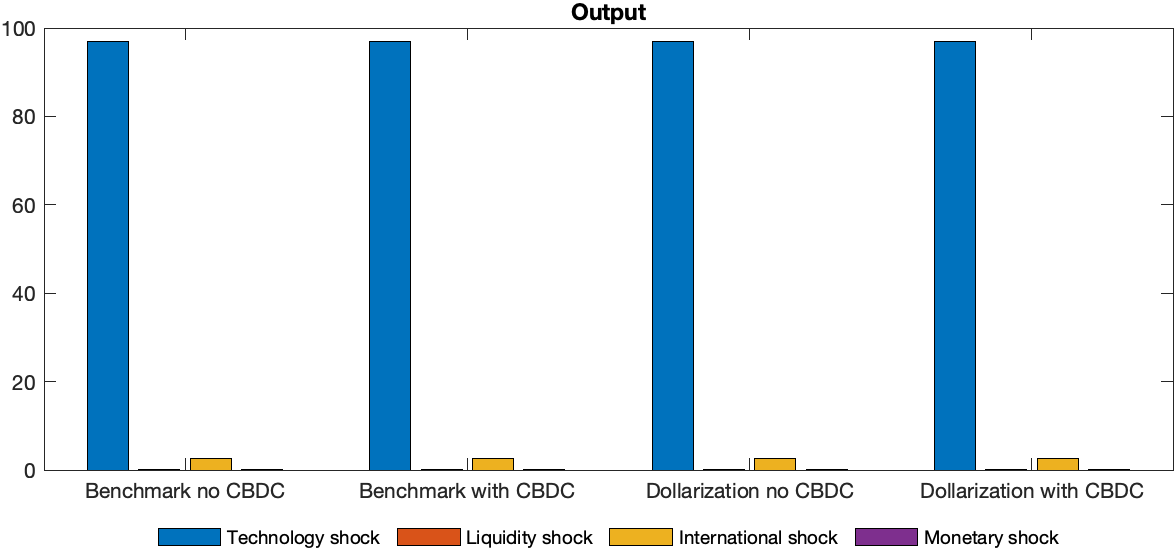
\includegraphics[width=0.8\textwidth]{log_y}
\end{figure}

\begin{figure}[h!]
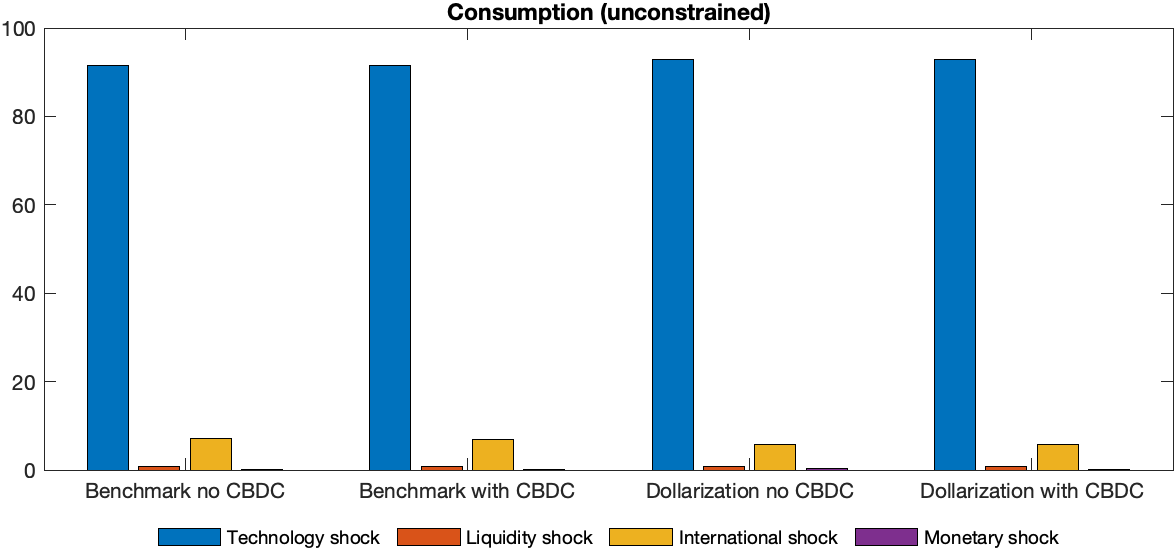
\includegraphics[width=0.8\textwidth]{log_c1}
\end{figure}

\begin{figure}[h!]
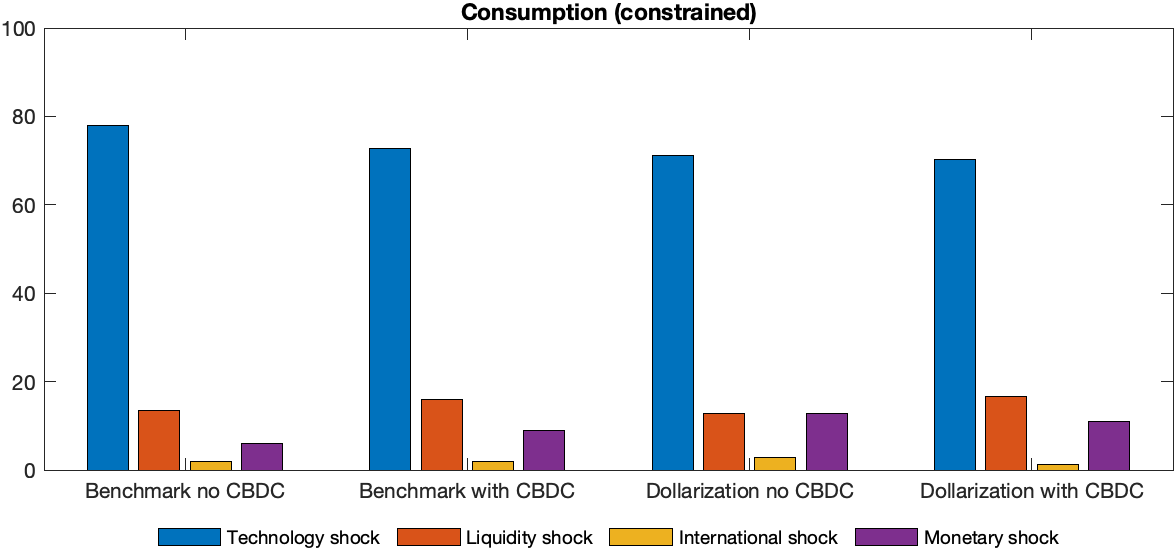
\includegraphics[width=0.8\textwidth]{log_c2}
\end{figure}

\begin{figure}[h!]
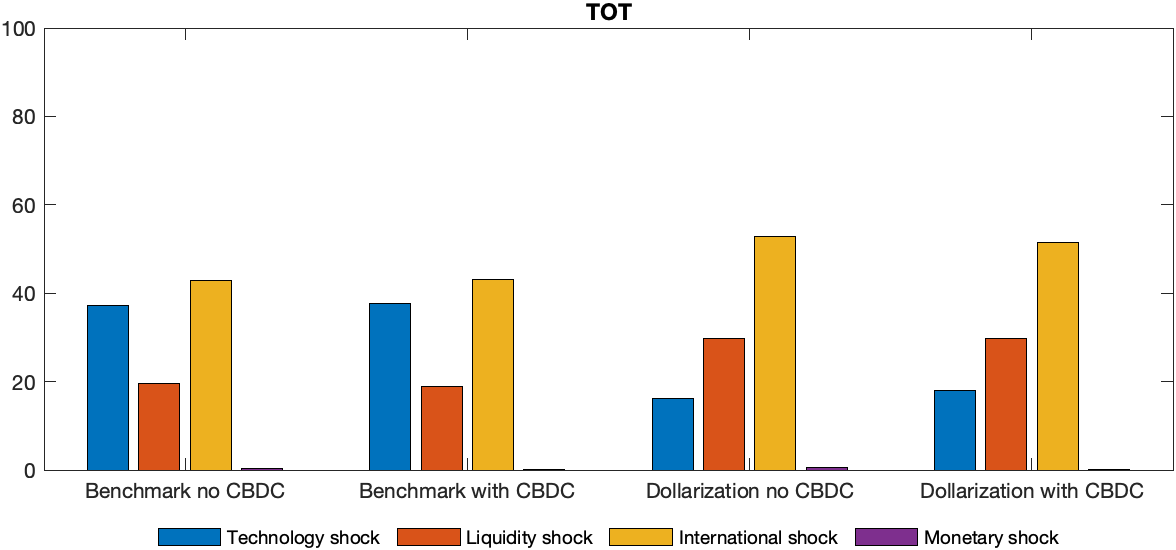
\includegraphics[width=0.8\textwidth]{log_tot}
\end{figure}


\clearpage
\section{Impulse Response}

\begin{figure}[h!]
\label{IRF1}
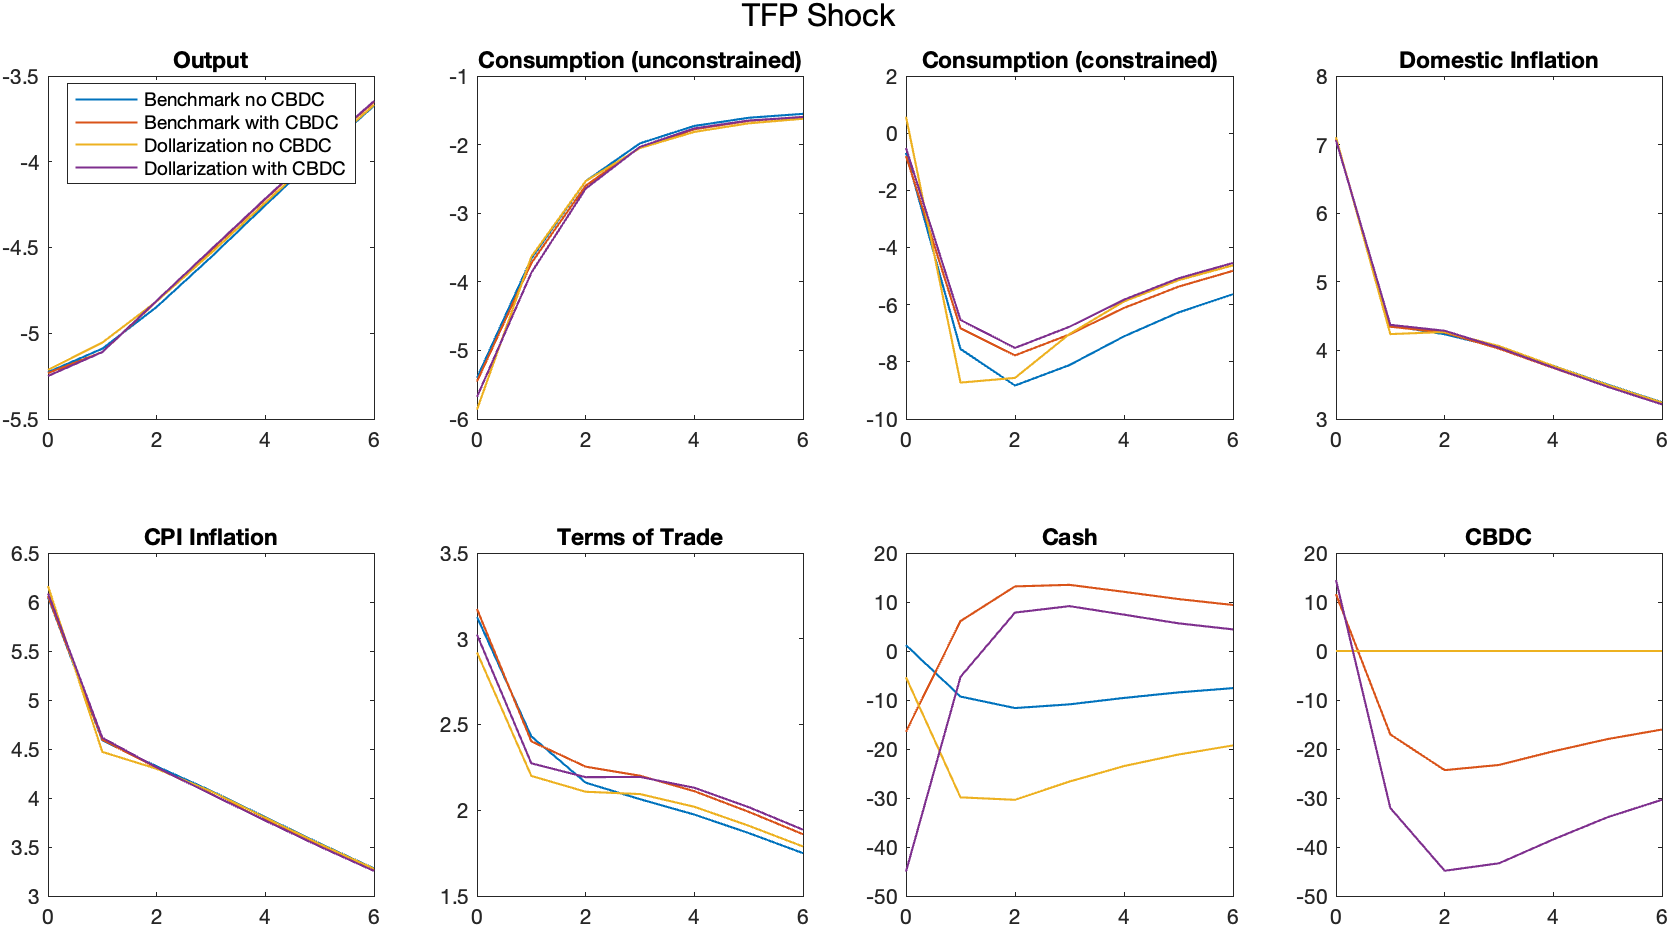
\includegraphics[width=\textwidth]{TFP}
\caption{Impulse Responses of TFP Shock}
\scriptsize{Notes: Response of key variables to a negative 1 standard deviation TFP shock. Vertical axes indicate percentage deviation from steady state. Horizontal axis indicate quarters after shock. }
\end{figure}
Figure \ref{IRF1} plots the responses of key variable following negative TFP shock. Introduction of CBDC decreases the responses of output and consumption to TFP. CBDC promotes financial inclusion of constrained household, and decreases the volatility of output and consumption. The terms of trade decreases following a negative TFP shock without CBDC, while it increases when CBDC is introduced. The constrained households switch more to cash following a negative TFP shock, since they are more sensitive to the consumption tax. 

\begin{figure}[h!]
\label{IRF2}
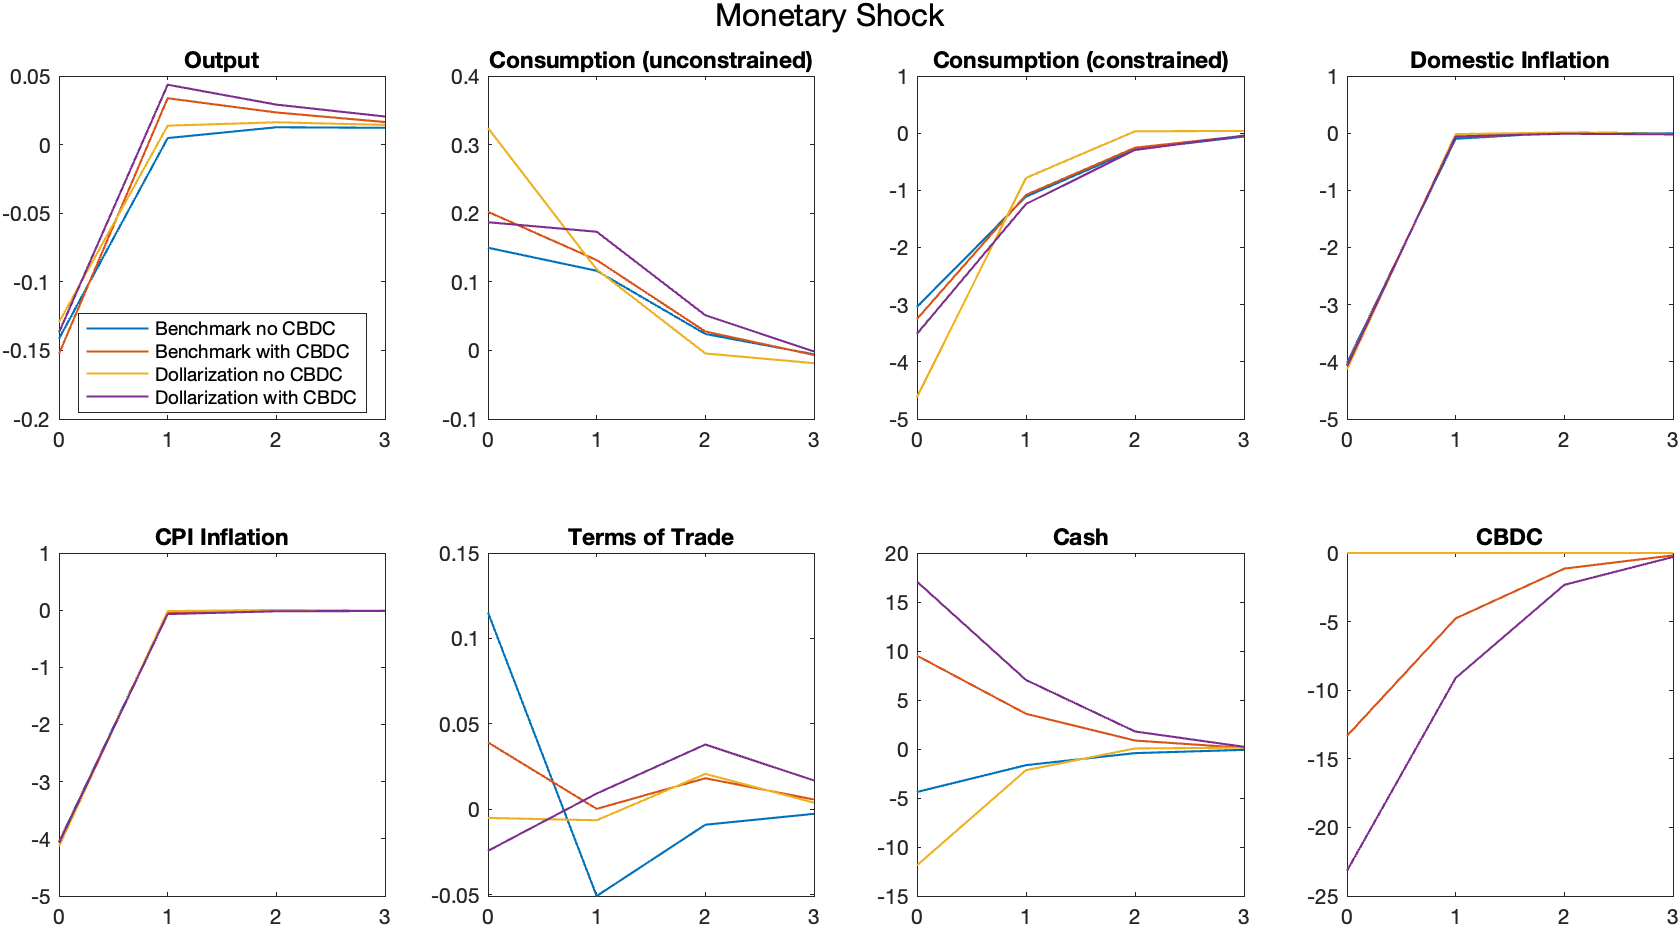
\includegraphics[width=\textwidth]{Monetary}
\caption{Impulse Responses of Monetary Policy Shock}
\scriptsize{Notes: Response of key variables to a positive 1 standard deviation monetary policy shock. Vertical axes indicate percentage deviation from steady state. Horizontal axis indicate quarters after shock. }
\end{figure}

\begin{figure}[h!]
\label{IRF3}
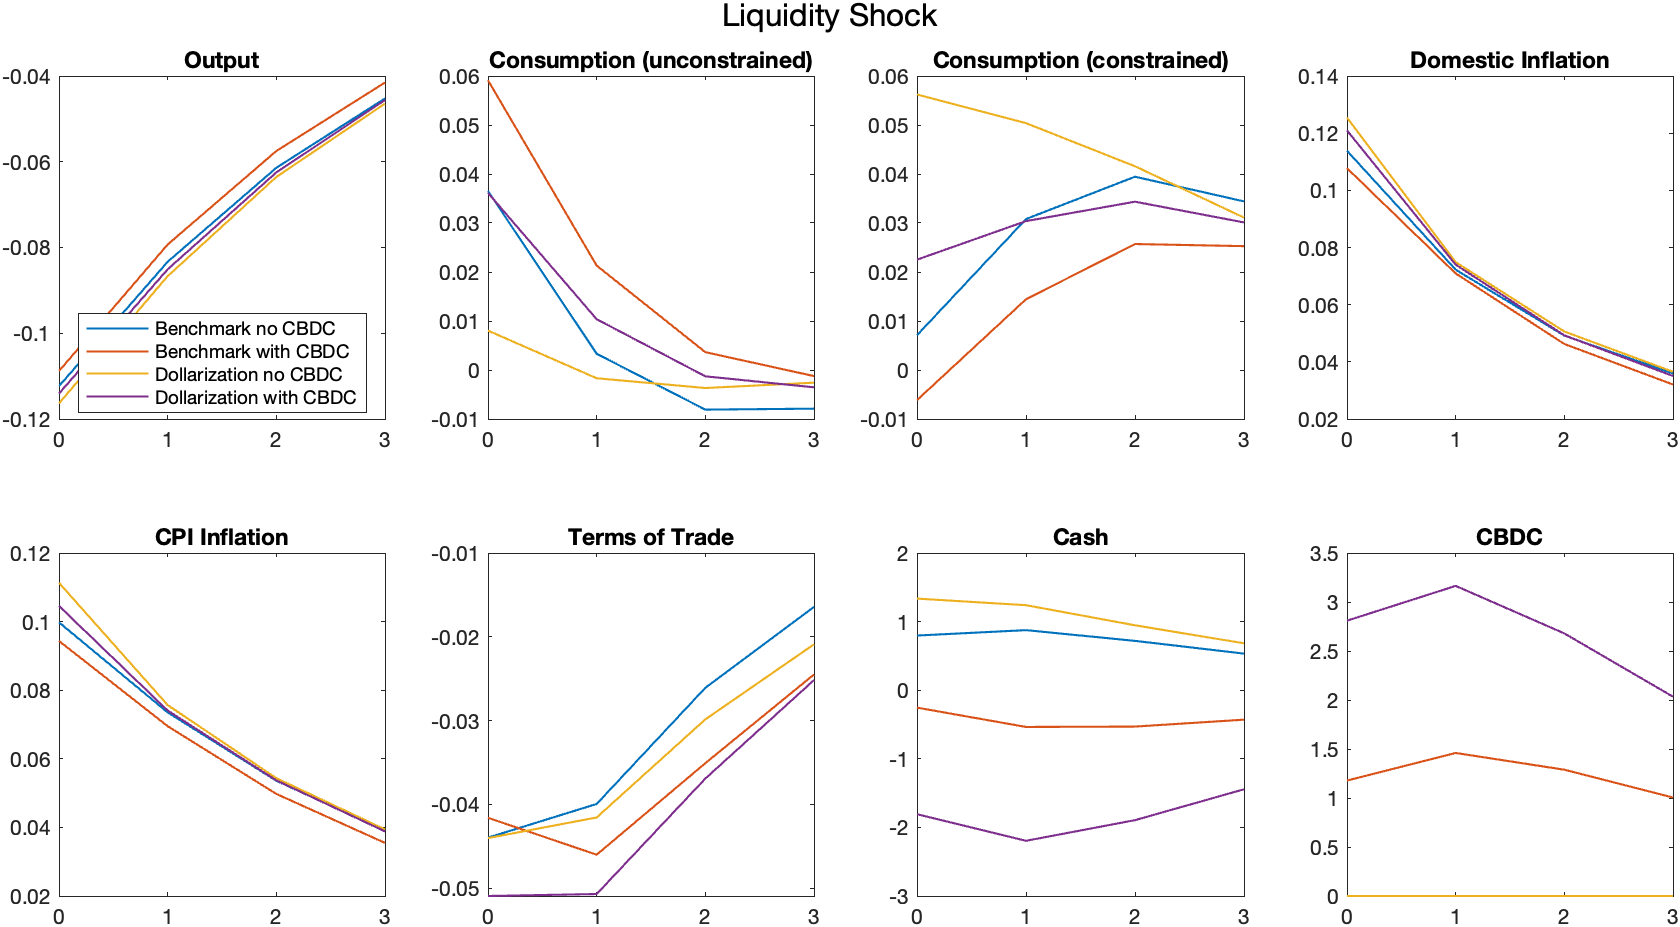
\includegraphics[width=\textwidth]{Liquidity}
\caption{Impulse Responses of Liquidity Shock}
\scriptsize{Notes: Response of key variables to a positive 1 standard deviation liquidity shock. Vertical axes indicate percentage deviation from steady state. Horizontal axis indicate quarters after shock. }
\end{figure}


\end{document}